\answer{What is a Java servlet?}{2}{2012.1.a}

A Java Servlet is a Java program with the capabilities of a server. It could
host web pages, provide an API endpoint or other services and is most commonly
used to serve content via the \texttt{HTTP} protocol.

\answer{What is the main assumption on which Cristian’s clock synchronisation
algorithm is based?}{2}{2012.1.b}

The time for a message to go from machine A to machine B is (roughly) the same
as the time it would take for a message to go from machine B to machine A. This
is most often accurate for routes with small round trip times.

\answer{Explain the difference between a name server and a directory
server.}{2}{2012.1.c}

A name server takes a name, matches it to an object and returns attributes about
the object. A directory server takes attributes, matches them to an object and
returns more attributes about the object.

\answer{Explain briefly what is meant by the term middleware.}{2}{2012.1.d}

Middleware is software that sits between a client application and the operating
system. It provides services to the client application that the operating system
does not, such as RPC stubs.

It can also provide an abstraction from the OS to mask the heterogeneity of
platforms used in distributed systems (some apps will run on Windows, others on
Linux, some on x64, some on ARM architectures etc).

\answer{Why is it practically impossible to achieve strict consistency in a
distributed  system?}{2}{2012.1.e}

Strict consistency is when any read to a shared data item returns the most
recent write operation on that data item. This means there must be an absolute
time ordering of all accesses. Unfortunately, since (as we know from the eight
fallacies of Distributed Computing), the latency of any network is not zero and
messages are not reliable. This means that any message we send to update other
machines about a change of state may not be sent. Since there is no way of
getting an absolute global clock or getting any global state, then we cannot
achieve real time memory consistency across all nodes, and therefore cannot
achieve strict consistency in the system.

\answer{Traditional RPC mechanisms cannot handle pointers. What is the
problem?}{2}{2012.1.f}

In order to handle pointers with RPC, you must serialise the datastructure into
a message so that it can be constructed from the same message at the other
machine. When the reply is received back at the sender, it can be deserialised
again and the values in the datastructure that were changed on the remote
machine can be updated in local memory. Traditional RPC mechanisms didn't have
this facility.

\answer{What is meant by parameter unmarshalling?}{2}{2012.1.g}

Extracting the parameters from an RPC message (can be binary data, ascii etc)
that was sent from another machine into memory of the local machine.

\answer{What is the key difference between caching and replication}{2}{2012.1.h}

Replication is keeping two fully fledged entities up to date with each other in
order to provide redundancy or distribute the load of a service over more
machines.

Caching is merely a small piece of hardware or a small program that remembers
the results of expensive computations after they've been done once and returns
the result without doing any computation if the same request comes again. Rarely
is there any business logic in a cache.

\answer{Explain briefly why somebody would like to use Cloud
Computing.}{2}{2012.1.i}

\begin{itemize}
  \item You don't have to buy and own hardware, you can just rent time from
    other people's hardware to do computing.
  \item Clouds are large and therefore provide capacity for horizontal scaling.
  \item Clouds make it easier to have the computing resources to apply
    techniques such as load balancing, replication and parallelization. This
    can make it easier to cope with variable demand.
\end{itemize}

\answer{In the context of lab exercise 2, what would you do to launch a denial 
of service attack against the server?}{2}{2012.1.j}

I would find the most computationally expensive operation on the server (maybe
list free slots, since it access the database a lot) and set up a tight loop to
continuously send requests for this operation to the server. To increase the
impact of my attack, I would try and execute it on a machine with a high network
bandwidth and low latency, as well as possibly using multiple threads or
machines to launch the attack.

\answer{Explain briefly what is wrong with the assumption “latency is zero” in
the context of distributed computing. Why is it considered a common
fallacy?}{3}{2012.2.a}

The latency between two computers can never be zero, for a number of reasons.
From a purely physical standpoint, information cannot travel faster than the
medium through which it is being carried, and even the fastest medium available
to us, light has a speed limit. Most of the time, latency is significantly
greater than the speed of light divided by the distance travelled, which is
because most of the time, the data passes through a network as packets, and is
forwarded on from node to node each time. Since multiple computers are used to
facilitate this, each one having some small amount of lag, the time between the
start point and the destination increases further. At any point along its route,
the data could get stuck in a buffer, have to take a detour etc.

Many (new) programmers haven't created applications intended to use distributed
systems before, and thus don't realise that waiting for a remote resource, RPC
call etc can (will) take orders of magnitude more time than a load from memory
might.

\answer{Explain briefly what the four properties commonly denoted by the acronym
ACID are when referring to transactions.}{3}{2012.2.b}

\begin{description}
  \item \textit{Atomicity} - Each operation/transaction must either succeed or 
  fail; there is no in-between. If the operation fails, then the state of the
  system must be exactly as it was before the start of the operation.
  \item \textit{Consistency} - Each operation or transaction must bring the
  state of the system from one valid state to another.
  \item \textit{Isolation} - Operations or transactions happening in parallel
  must execute as though they were running in a serial manner.
  \item \textit{Durability} - Once a transaction is committed or an operation
  is completed, the system will not roll back to a previous state in the event
  of failure or power loss etc.
\end{description}

\answer{Outline the Byzantine Generals problem, and illustrate how one of three
being a traitor makes a solution impossible, whereas with one of four it is
achievable.}{6}{2012.2.c}

There are three Byzantine generals on the battlefield. One is the commander and
the other two are his deputies. Each of the `good' generals knows that the
others could be corrupt, but not which one (or any of them). In order to make
sure they never do the wrong thing, they agree that a commander must receive the
same message from both other commanders before he does anything.

However, if one commander is corrupt, they can change every message they receive
and make it so that the other two commanders will never do anything since the
other two commanders will always receive conflicting messages.

However, if there is one corrupt commander within four (or more) commanders,
then they can never cause a deadlock like that, because they will always be a
minority among the other non-corrupt commanders.

\answer{The following four processes access a shared variable x. Each process
accesses a different replica of the store used to hold this variable. Before any
process starts executing, the value of x is 0 in all the replicas.}{8}{2012.2.d}

\begin{center}
  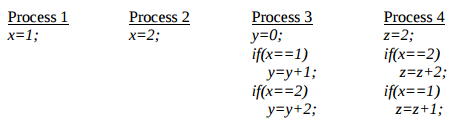
\includegraphics[width=0.5\textwidth]{images/2012-2-d}
\end{center}

\answer{When all four processes have completed executing the statements
given, are 3 and 5 possible values of y and z respectively, if the
replication uses the sequential consistency model? Justify your
answer.}{4}{2012.2.d.i}

No, because for $y=3$ and $z=5$, the values of $x$ must change during the
execution of process 3 and process 4. This cannot occur in a sequential
consistency model, since each process must run one after another, and process 3
and 4 don't change the value of $x$.

\answer{When all four processes have completed executing the statements
given, are 3 and 5 possible values of y and z respectively, if the
replication uses the causal consistency model? Justify your
answer.}{4}{2012.2.d.ii}

No, since for $y=3$ and $z=5$ require all of the if statements to evaluate to
true and execute all of the additions, since $0 + 1 + 2 = 3$ and $2 + 2 + 1 =
5$. Since process 3 requires $x$ to be 1 first and process 4 requires it to be 2
first, we can only ever get three of the four if statements to execute. This
means we can get either $y=3$ or $z=5$ (or none of them), but not both.

\answer{Explain briefly what is the role of a client stub and a server stub in
RPC}{3}{2012.3.a}

A stub is middleware that sits between an application and the OS. Its role is to
facilitate an RPC call, but its exact `job description' varies based on whether
its a client or server stub:

\begin{description}
  \item \textbf{Client}:
    \begin{enumerate}
      \item First, the stub will marshal the parameters to the remote method
        into a text or binary format.
      \item The client stub then sends the request to the server (where the
        server stub will handle it) and waits for a reply.
      \item Once it receives a reply the client stub unmarshals the data from
        the servers reply back into memory and returns back to the client
        application.
    \end{enumerate}
  \item \textbf{Server}:
    \begin{enumerate}
      \item When the server receives a message from a client sub, it unmarshals
        the parameters and puts them in memory.
      \item Then it calls the desired procedure on the server application
      \item When the procedure has finished, it marshals the data back into a
        message and sends it back to the client.
    \end{enumerate}
\end{description}

\answer{Describe in detail how the two-phase commit protocol can implement
distributed transactions}{5}{2012.3.b}

\begin{itemize}
  \item There is a server that acts as a coordinator.
  \item When a client wants to commit a transaction, it sends a message to the
    server asking to commit.
  \item The server then sends a message to all clients asking if they are in a 
    state where they can commit.
  \item Each client sends a reply (either yes or no) as to whether they can
    commit.
  \item If all of the clients are in a position to commit, then the server will
    send out a \texttt{global\_commit} message and all clients will commit, 
    otherwise, it will send out a \texttt{global\_abort} message and all clients
    will abort the transaction.
\end{itemize}

\answer{Consider the figure below, which shows 4 processes and a number of
communication events taking place over a period of time. Calculate the value of
Lamport clocks and vector clocks for each of the 12 events. You can assume that
all logical clocks start initially with zeros.}{6}{2012.3.c}

\begin{center}
  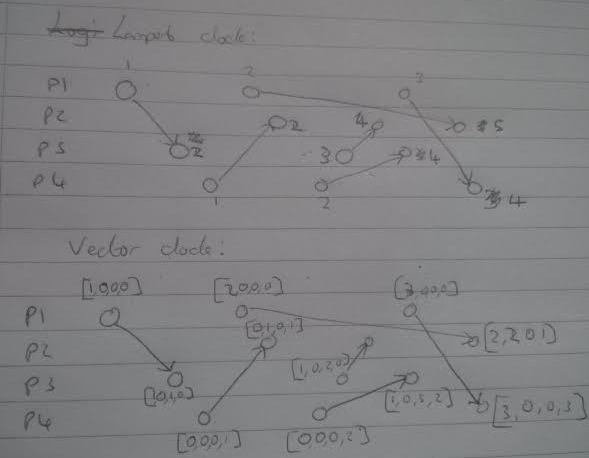
\includegraphics[width=0.6\textwidth]{images/2012-3-d}
\end{center}

\answer{In a system containing 7 computers, identified by the integers 1-7, the
coordinator is chosen by the Bully algorithm to be the live one with the
highest identifier. Assume for this part that all messages are delivered
promptly, and that the computers and the network are entirely reliable.
At a certain point in time the coordinator (computer 7) and the computer with
the second-highest identifier (computer 6) crash. How many messages in total
are sent if the computer with identifier 1 is the computer discovering the crash
and triggering an election? You need to count all three types of messages that
the algorithm sends. You can assume that computers with identifiers 6 and 7
remain crashed during the election.}{6}{2012.2.d}

First, 1 will send a message to all computers higher than it ($2,3,4,5,6,7$)
totalling six messages. Each live process receiving a message from 1 will then
send messages to processes higher than it:

\begin{center}
  \begin{tabular}{cl}
    \textbf{Computer} & \textbf{Election messages sent}\\
      1 & $2,3,4,5,6,7$\\
      2 & $3,4,5,6,7$\\
      3 & $4,5,6,7$\\
      4 & $5,6,7$\\
      5 & $6,7$\\
      6 & Crashed!\\
      7 & Crashed!
  \end{tabular}
\end{center}

This totals $6 + 5 + 4 + 3 + 2 = 20$ messages sent.

Each process then receives a reply from the live ones above it:

\begin{center}
  \begin{tabular}{cl}
    \textbf{Computer} & \textbf{Replies received}\\
      1 & $2,3,4,5$\\
      2 & $3,4,5$\\
      3 & $4,5$\\
      4 & $5$\\
      5 & \\
      6 & \\
      7 & \\
  \end{tabular}
\end{center}

This totals $4 + 3 + 2 + 1 = 10$ messages.

The winner of the election ($5$) then sends a message to all other processes to
announce its win (five more messages), so a total of $20 + 10 + 5 = 35$ messages
are sent.
